\documentclass[preview]{standalone}

\usepackage{amsmath}
\usepackage{amssymb}
\usepackage{stellar}
\usepackage{bettelini}

\hypersetup{
    colorlinks=true,
    linkcolor=black,
    urlcolor=blue,
    pdftitle={Biologia},
    pdfpagemode=FullScreen,
}

\begin{document}

\title{Biologia}
\id{biologia-trasmissione-delle-informazioni}
\genpage

\plain{La trasmissione delle informazioni viene trasmessa mediante un impuslo elettrico
che viaggia in una sola direzione.}

\begin{snippet}{potenziale-riposo}
    \textbf{Potenziale di riposo:} in un neurone a riposo, ovvero che non sta conducendo nessun impulso, il citoplasma
all'interno della membrana plasmatica ha una carica negativa netta rispetto al liquido
interstiziale all'esterno, pari a -70 mV. Il potenziale di riposo è generato dalla diversa
composizione e concentrazione degli ioni presenti all'interno e all'esterno della cellula. Nel
citoplasma del neurone i principali cationi sono il sodio Na\({}^+\) e il potassio K\({}^+\). Nella maggior
parte dei neuroni la concentrazione del potassio è elevata dentro la cellula, mentre quella
del sodio è elevata all'esterno della cellula. Questo è dovuto alla pompa sodio potassio,
ovvero proteine di membrana che utilizzano energia per trasportare attivamente ioni Na\({}^+\)
all'esterno della cellula e ioni K\({}^+\) all'interno. Una membrana a riposo presenta molti canali
ionici aperti per la diffusione del K\({}^+\) e solo pochi per il Na\({}^+\). Di conseguenza, gli ioni K\({}^+\)
diffondono spontaneamente verso l'esterno, assecondando il proprio gradiente di
concentrazione, più di quanto facciano gli ioni Na\({}^+\) verso l'interno della cellula. Poiché il
movimento degli ioni corrisponde a un movimento di carica elettrica, la fuoriuscita degli ioni
K\({}^+\) (positivi) determina la formazione di una carica netta negativa all'interno della cellula.
\end{snippet}

\begin{snippet}{neurone-membrana-illustration}
    \begin{center}
    \begin{figure}[ht]
        \centering
        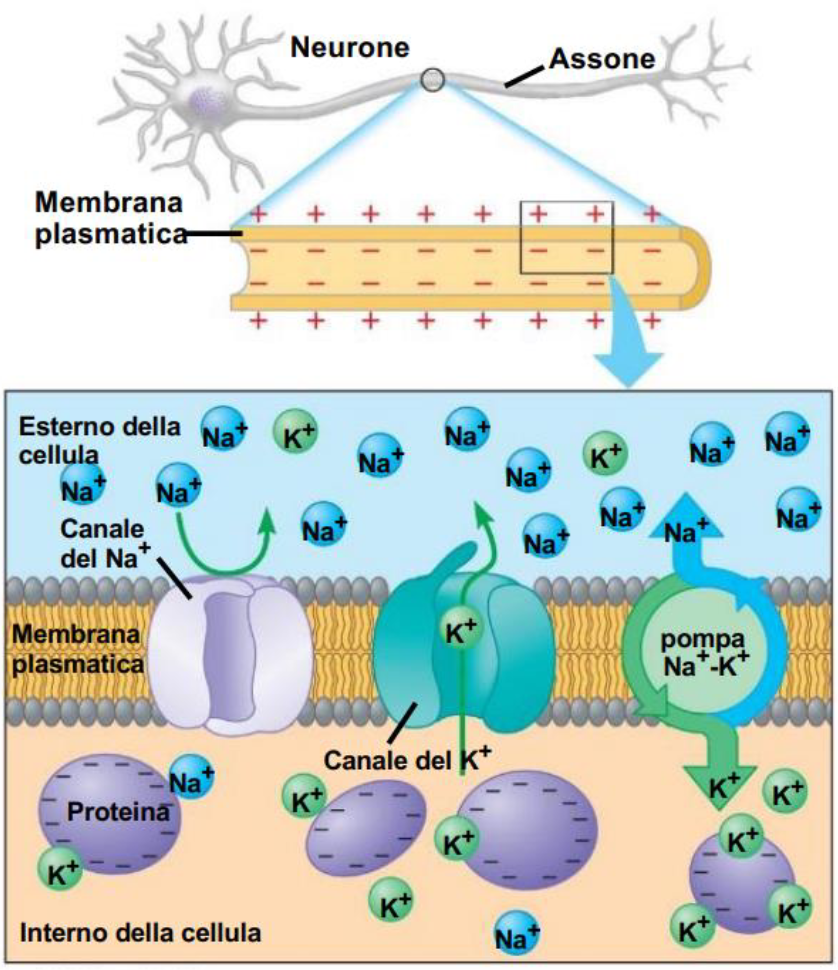
\includegraphics[width=0.75\textwidth]{./resources/neurone_membrana.png}
    \end{figure}
    \end{center}
\end{snippet}

\begin{snippet}{potenziale-azione}
    \textbf{Potenziale di azione:} Si tratta del segnale nervoso che trasporta l'informazione lungo l'assone.
In condizioni di riposo, la membrana plasmatica separa l'ambiente esterno, carico positivamente, da quello
interno, carico negativamente. Quando uno stimolo determina l'apertura di alcuni canali
voltaggio dipendenti del Na\({}^+\), una piccola quantità di ioni Na\({}^+\) entra nell'assone. Ciò
comporta una leggera depolarizzazione della superficie della membrana. Se lo stimolo è
abbastanza intenso, il numero di canali del Na\({}^+\) che si apre è tale da portare il potenziale di
membrana al valore soglia, ovvero -50 mV. Una volta raggiunta la soglia, si aprono altri
canali voltaggio dipendenti del Na\({}^+\), permettendo ad altri ioni sodio di fluire dentro la cellula.
Man mano che questo accade, il potenziale di membrana raggiunge il potenziale d'azione,
che innesca la chiusura e la disattivazione dei canali voltaggio dipendenti del Na\({}^+\). Si aprono
i canali del K\({}^+\) permettendo agli ioni potassio di diffondere rapidamente all'esterno; quindi,
la cellula torna ad essere carica negativamente all'interno. Poiché i canali del K\({}^+\) si chiudono
lentamente, si ha una breve caduta del potenziale di membrana al di sotto del potenziale di
riposo. La membrana, infine, ritorna nella condizione di riposo.
\end{snippet}

\begin{snippet}{f5877579-81ce-44fc-a3b7-7dd846d264ce}
    Possiamo quindi schematizzare questi processi nella seguente maniera:
    \begin{enumerate}
        \item \textbf{condizione a riposo:} i canali voltaggio dipendenti del Na\({}^+\) e del K\({}^+\) sono chiusi e il potenziale
            è mantenuto dai canali ionici a -70 mV;
        \item \textbf{depolarizzazione:} uno stimolo provoca l'apertura di alcuni canali del Na\({}^+\). Se viene raggiunto
            il potenziale soglia di -50 mV, si genera il potenziale d'azione;
        \item si aprono altri canali del Na\({}^+\), i canali del \({}^+\) sono chiusi e l'interno della cellula diventa più
            positivo;
        \item \textbf{ripolarizzazione:} i canali del Na\({}^+\) si chiudono, mentre si aprono quelli del K\({}^+\) che fluisce
            all'esterno. L'interno della cellula torna ad essere più negativo dell'esterno;
        \item i canali del K+ si chiudono lentamente, provocando una breve caduta al di sotto del
            potenziale di riposo.
    \end{enumerate}
\end{snippet}

\begin{snippet}{grafico-potenziale-illustration}
    \begin{center}
    \begin{figure}[ht]
        \centering
        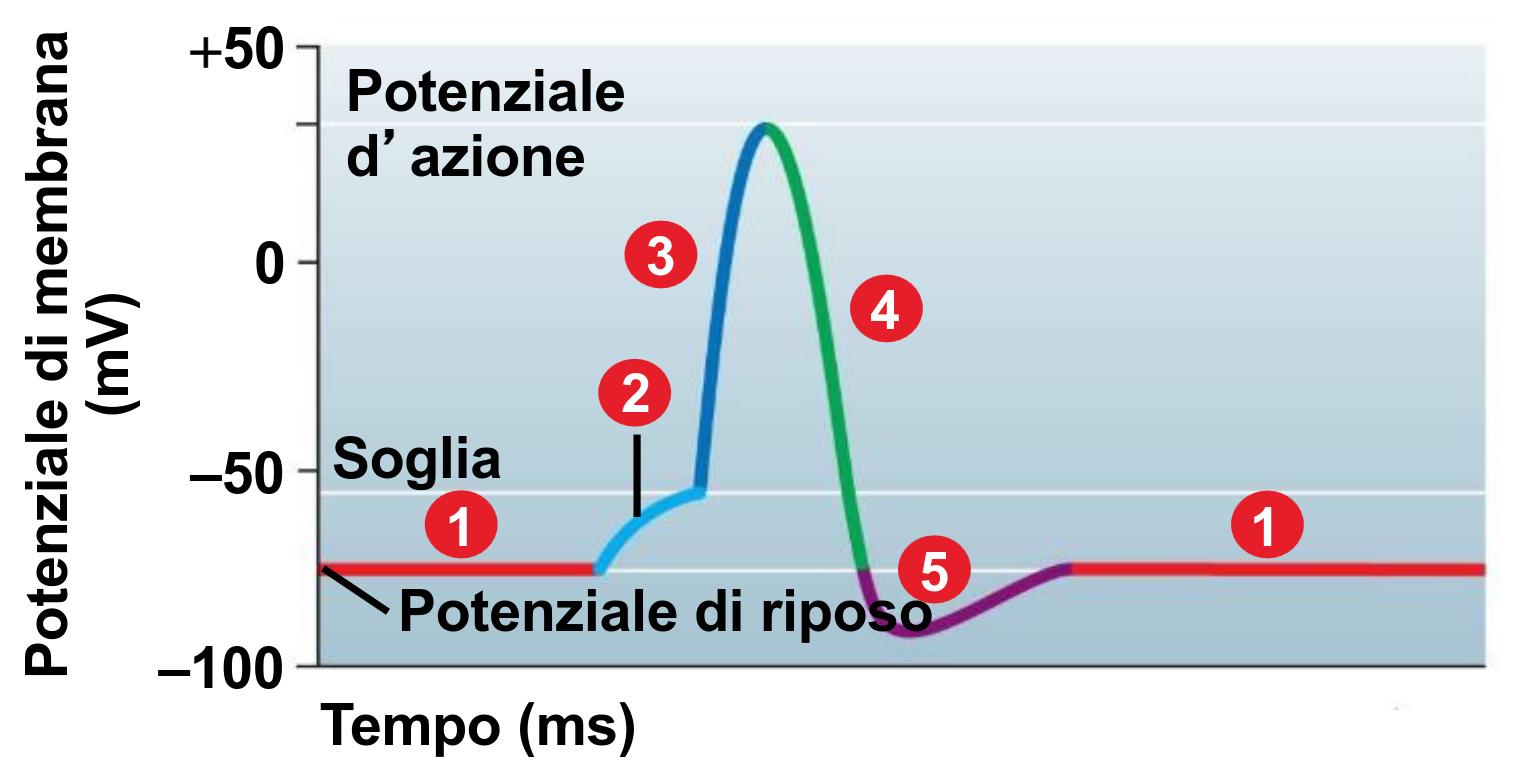
\includegraphics[width=0.6\textwidth]{./resources/grafico_potenziale_membrana_neurone.png}
    \end{figure}
    \end{center}
\end{snippet}

\section{Comunicazioni fra neuroni}

\begin{snippetdefinition}{sinapsi-elettriche-definition}{Sinapsi elettriche}
    La trasmissione del segnale nervoso avviene per passaggio diretto di ioni da un neurone
    all'altro, tramite le giunzioni comunicanti, che collegano le membrane dei due neuroni
    coinvolti. Questo tipo di trasmissione è molto veloce e bidirezionale.
\end{snippetdefinition}

\begin{snippetdefinition}{sinapsi-chimiche-definition}{Sinapsi chimiche}
    Il neurone presinaptico secerne un neurotrasmettitore, che attraversa la fessura sinaptica
    e si lega a un recettore sulla membrana della cellula postsinaptica.
\end{snippetdefinition}

\begin{snippet}{90f332b6-c3ee-4a69-954c-81170905e5b9}
    \begin{itemize}
        \item  La \textit{sinapsi elettrica} è presente quado il segnale nervoso passa direttamente dal
        neurone presinaptico alla cellula successiva, detta postsinaptica (il bottone fonde con la cellula che viene dopo).
        \item La \textit{sinapsi chimica}
        \begin{itemize}
            \item Il neurone presinaptico secerne un neurotrasmettitore
            \item Il neurotrasmettire attraversa la fessura sinaptica
            \item Il neurotrasmettitore si lega ad un recettore sulla mebrana della cellula postsinaptica
        \end{itemize}
    \end{itemize}
\end{snippet}

\begin{snippet}{giunzione-sinapsi-illustration}
    \begin{center}
    \begin{figure}[ht]
        \centering
        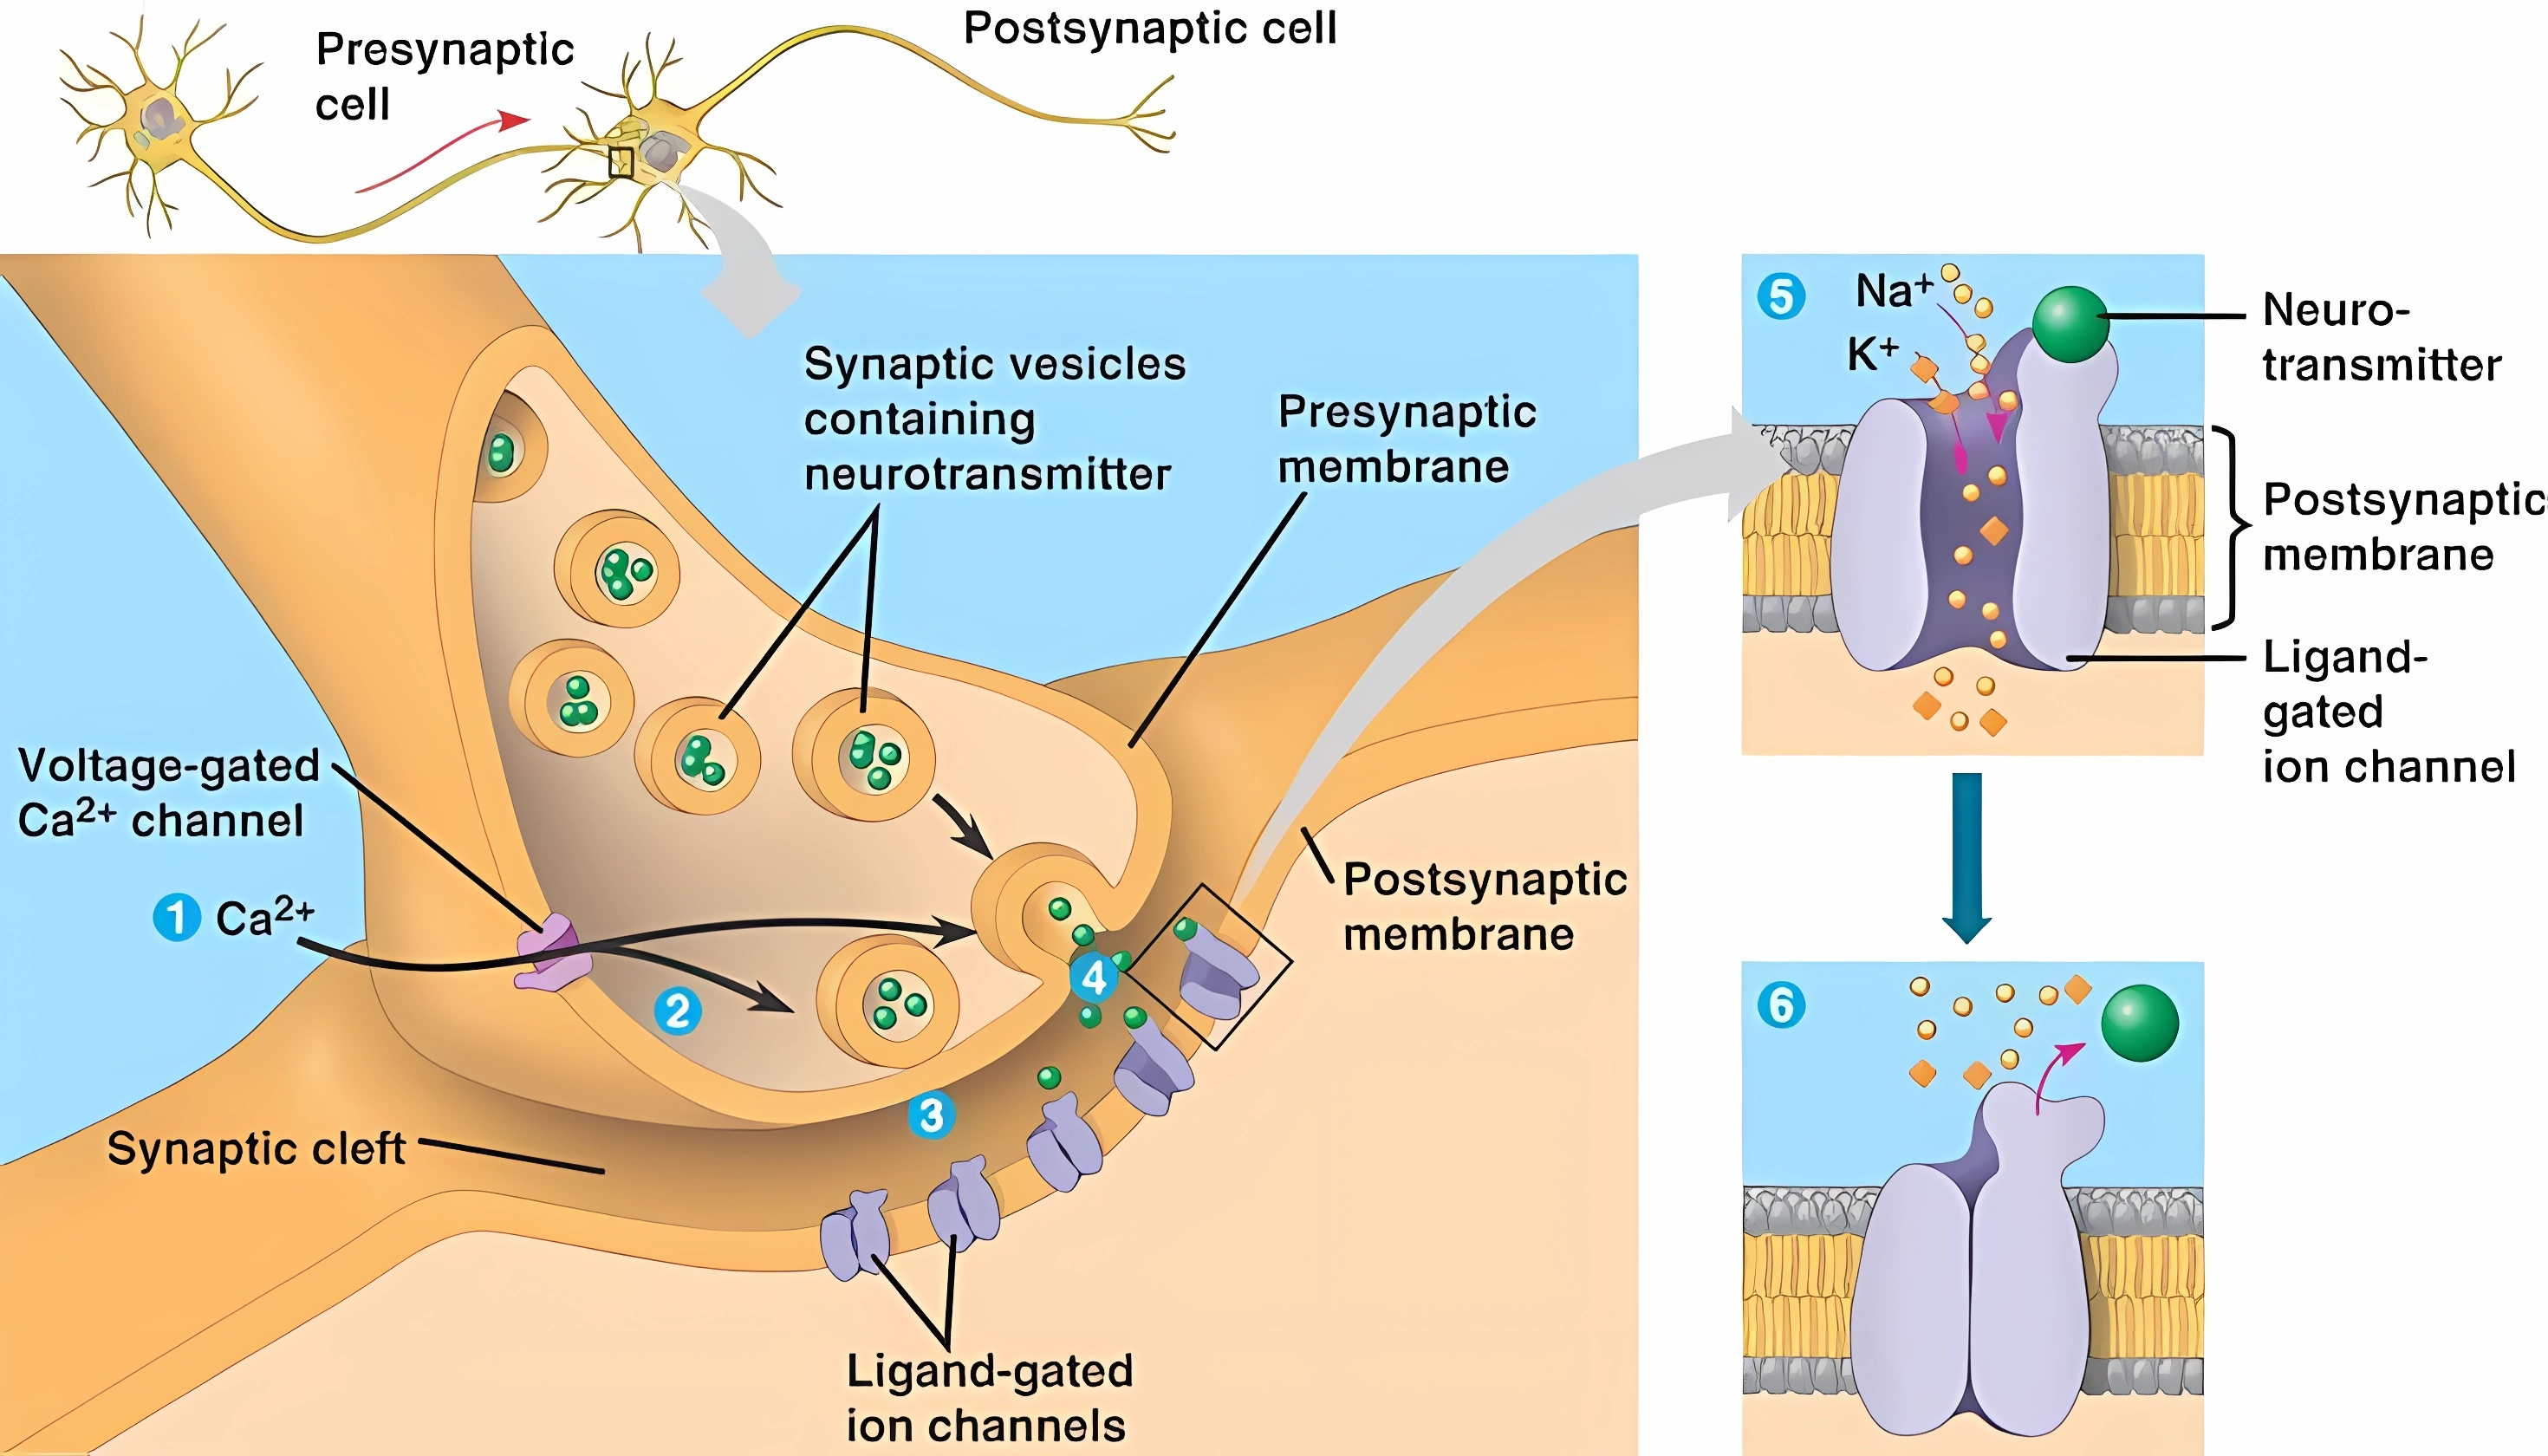
\includegraphics[width=0.9\textwidth]{./resources/giunzione_sinapsi.png}
    \end{figure}
    \end{center}
\end{snippet}

\begin{snippet}{01dd82bf-6b50-4791-ac3e-737d0e31eb75}
    \begin{enumerate}
        \item Quando arriva un potenziale d'azione, la membrana presinaptica si depolarizza;
        \item La depolarizzazione apre i canali voltaggio dipendenti per il calcio Ca\({}^{2+}\) nella membrana
            presinaptica; dunque, un flusso di ioni Ca\({}^{2+}\) entra nella cellula.
        \item L'elevata concentrazione di calcio induce la fusione delle vescicole sinaptiche con la
            membrana presinaptica, determinando il rilascio del neurotrasmettitore nella fessura
            sinaptica.
        \item La fusione della vescicola sinaptica con la membrana presinaptica determina il rilascio del
        neurotrasmettitore nella fessura sinaptica.
        \item Il neurotrasmettitore si lega ai recettori presenti sulla membrana postsinaptica.
        \item In seguito, viene demolito o riassorbito per endocitosi.
    \end{enumerate}
\end{snippet}

\begin{snippet}{eccitatori-inibitori-expl}
    I segnali possono essere eccitatori o inibitori.
Quelli eccitatori voglio far partire il segnale, mentre quelli inibitori
fermarlo. Quello che fa stato è il risultato, ossia la somma di tutte
all'inizio dell'assone.
\end{snippet}

\begin{snippetdefinition}{neurotrasmettitore-definition}{Neurotrasmettitore}
    I \textit{neurotrasmettitori} sono sostanze prodotte dai neuroni e liberate nelle sinapsi (più
    esattamente nello spazio o fessura sinaptica) in seguito all'arrivo di un impulso nervoso.
    \begin{itemize}
        \item \textit{neurotrasmettitori eccitatori:} determina una depolarizzazione della membrana post-sinaptica;
        \item \textit{neurotrasmettitori inibitori:} determina una iperpolarizzazione della membrana.
    \end{itemize}
\end{snippetdefinition}

\begin{snippetdefinition}{seratonina-definition}{seratonina}
    La \textit{seratonina} è un neurotrasmettitore inibitorio.
\end{snippetdefinition}

\begin{snippet}{07a4ccb4-d8a7-46c7-99e3-d9ffc85cd693}
    La seratonina apre dei canali come quelli del potassio per inibire un determinato percorso.
L'inibizione di questo neurone postsinaptico è in un contesto che aiuta la felicità.
\end{snippet}

\end{document}